\documentclass[twoside,11pt,ShortChapTitles]{BYUTextbook}

\usepackage{soul}
\renewcommand{\vec}[1]{\ensuremath{\mathbf{#1}}}
\newcounter{dummy}
\usepackage[style=verbose,backend=bibtex]{biblatex}  % For footnote citations
\addbibresource{refs.bib}
\usepackage[super]{nth}
\newcommand{\labsection}[1]{\refstepcounter{dummy}\addcontentsline{toc}{section}{#1}\section*{#1}}
\usepackage{siunitx}
\sisetup{round-mode = figures,
  round-precision = 3, scientific-notation=true}
\newif\ifsolutions
\solutionsfalse

\begin{document}

\frontmatter

 \thispagestyle{empty}
 \begin{adjustwidth}{}{-1.5in}
 \centering
 {\huge Machine Learning for Physicists}
 %\vskip1.5truein

    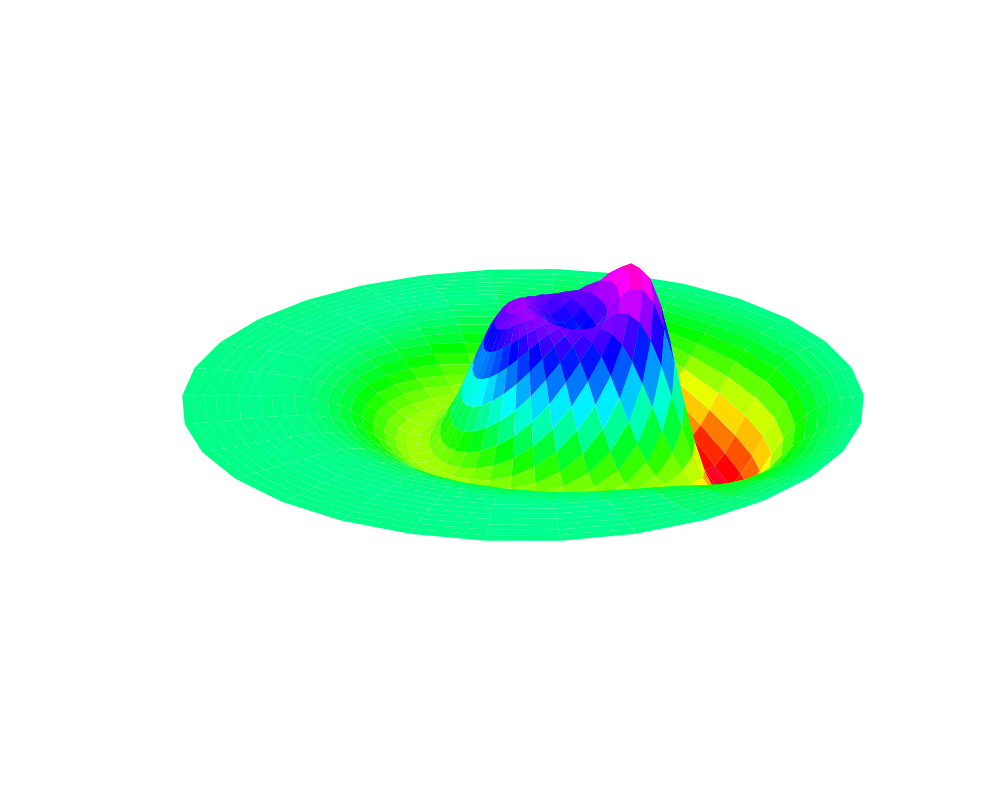
\includegraphics[scale=0.6]{Figures/circMembrane}

%\vskip1truein
Lance J.\ Nelson

\vskip.4truein
Department of Physics
\end{adjustwidth}

\cleardoublepage
\thispagestyle{empty}

 \begin{adjustwidth}{}{-1.5in}
 \centering
 \vspace*{1in}
 \large
 {\huge Machine Learning for Physicists}
 \vskip.4truein

 Lance J.\ Nelson
 \bigskip

 Department of Physics

 \bigskip
 Brigham Young University--Idaho

 \vfill


 {\footnotesize $\copyright$ 2020 Lance J.\ Nelson
               Brigham Young University--Idaho}

 \vskip.5truein
 {\footnotesize \emph{Last Revised: \today}}
 \normalsize

 \end{adjustwidth}

\cleardoublepage
\phantomsection
\chapter*{Preface}

This is a lab notebook intended to give you experience solving
ordinary and partial differential equations numerically.  The
objectives of this course are 
\begin{itemize}
\item to help you learn how to solve a differential equation
  numerically; in situations when a paper-and-pencil solution is
  impossible or impractical.
\item to help you gain greater skills programming a computer and using
  loops, logic, functions, and classes.
\item that your ability to produce a high-quality, professional
  scientific document will increase.
\end{itemize}

Text with a bold P designation (\textbf{P1.1} for example) indicate tasks
that will be done together in class.  Text with a bold H designation
are homework problems and should be completed out of class. (working
in groups is encouraged.) 

Python is the programming language that we will be using You can
obtain a free copy of Python
\href{https://store.enthought.com/downloads/}{here}.  Any computer
code that you create should be uploaded to the Google Drive folder
provided.

There is a companion book to this one entitled, ``Introduction to
Python''.  It is intended to help you learn to use Python to do the
tasks contained herein.  


 \cleardoublepage 
\phantomsection
 \addcontentsline{toc}{chapter}{Table of Contents}
\tableofcontents

\mainmatter
\renewcommand{\chaptermark}[1]{\markboth{Computational Physics 385}{\chaptername \ \thechapter \ \ #1}}
\part{Simple Probability}
\chapter{Introduction to Probability}
 \label{chap:probability} \index{Probability}
 \index{Kernels}

 \labsection{Simple Probability} For most people, the idea of simple
 probability is pretty intuitive.  The probability of rolling a 5 on a
 6-sided die is ${ 1\over 6}$ because of the $6$ possible outcomes,
 only one of them produces a $5$.  The probability of drawing a red
 card in a standard, 52-card deck is ${13\over 52}$ because of the 52
 total cards, $13$ of them are red.  Generalizing this idea yields the
 equation:

\begin{equation}\label{eq:simpleProb}
  P(\text{event~ A}) = {\text{\#~of~ways~A~can~happen}\over \text{Total~\#~of~things~that~could~happen}}
\end{equation}


This equation is the most general version for calculating probability
and is a good one to fall back on when you get stuck.  However,
sometimes it's hard, or impossible, to count the number of possible
outcomes. For example, consider rolling a fair, $6$-sided dice, three
times.  What is the probability that the sum of these three rolls is
less than $10$?  To answer the question using equation
\eqref{eq:simpleProb} you could write down all possible combinations
of three dice rolls (there are 216 of them) and then identify how many
of them summed to a number less than $10$.  While you could probably
write some computer code to do this fairly easily, you probably don't want to do
it by hand. If you're still skeptical, consider increasing the number
of dice rolls to 4 or 5 and reconsider the problem.  It isn't hard to get a
situation where brute-force enumeration and counting is not a great idea.


What follows are some tricks and rules that you can
use to calculate probability when brute-force counting is intractable.


\labsection{Probability of multiple events} 

For example, a single dice roll has $6$ possible outcomes, two dice
rolls has $36$ possible outcomes (illustrated in figure
\ref{twoDieRolls}) and three dice rolls has $216$ possible outcomes.
Clearly you don't want to be enumerating these by hand.  One scenario
where outcome counting becomes challenging is when asking about the
probability of multiple events occuring.  This is because you have to
consider whether the outcome of one event will affect the outcome of
the next.  For example, suppose you roll a $6$-sided die twice and you
want to know the probability that both rolls come up $5$.  Having a
$5$ come up on the first roll doesn't affect the probability that a
$5$ comes up on the second.  These two events are independent of one
another.  The outcome of one event does not affect the outcome of the
other.

In contrast, consider randomly selecting marbles out of a bag which initially
contains $3$ red marbles and $8$ green marbles.  If you reach into the
bag and grab two marbles, what is the probability that they will both
be red?  Notice that selecting a red marble on the first reach into the bag
modifies the number or red marbles available for selection on the
second reach into the bag. Hence the two probabilities are dependent
on each other.  This is an example of dependent events.

\subsection*{Intersection of two events (event A \underline{and} event B)}
\marginfig[-1in]{Figures/twoDieRollsII}{\label{twoDieRolls}All 36
  outcomes from rolling two fair dice.  Out of 36 possible outcomes,
  only one yields a $5$ on both rolls.  Hence the probability of
  rolling two $5$'s is ${1\over 36}$.}

We'll start with the case where two events, $A$ and $B$, both
occur. (Also called the intersection of two events. See figure \ref{fig:VennDiagram})
The math for this sort of situation is:

\begin{equation}
  P(A \cap B) = P(A)  \times P(B)\nonumber
\end{equation}

but let's see some examples so it makes more sense.


\subsubsection*{Independent Events}
Consider rolling a fair $6$-sided dice.  What is the probability that
$5$ comes up on the first two rolls?  Your intuition is probably telling
you that rolling two $5$'s is less likely than rolling just one, so
you expect the probability to be less than ${1\over 6}$.  In figure
\ref{twoDieRolls} you will see all 36 possible outcomes when rolling a
fair dice two times.  Of those 36 possible outcomes how many of
occurrences of two $5$'s being rolled were there?  Just one.  Hence,
the probability is ${1\over 36}$.  You may have noticed that
${1\over 36} = {1\over 6} \times {1\over 6}$.  In other words, the
probability of event A happening \textbf{and} event B happening is
just the product of the two individual probabilities:

\begin{equation}
  P(A\text{ and } B) = P(A) \times P(B)\nonumber
\end{equation}



sometimes $P(A\text{ and } B)$ is written using the symbol for
intersection ($\cap$):
\begin{equation}\label{eq:andprobability}
  P(A \cap B) = P(A) \times P(B)
\end{equation}




\subsubsection{Dependent Events}
When the outcome of one event is affected by the outcome of a previous
event, we say they events are dependent.  For example, consider a bag
containing $3$ red marbles and $8$ green marbles.  If I reach into the
bag and select two marbles, what is the probability that they are both
red.  The probability that my first selection is red is:

\begin{equation}
P(A) = {3\over 11}  \nonumber
\end{equation}

\marginfig[-1in]{Figures/VennDiagram}{\label{fig:VennDiagram}If the
  blue circle represents the probability of A occuring and the red
  circle represents the probability of B occuring, then the overlap of
these two circles is the probability of both events occuring. By
sliding one cirle left or right we can adjust the size of the overlap
(aka $P(A|B)$)}

because $3$ out of the $11$ choices are red.  What about the second
selection?  After the first selection, I am left with $10$ marbles,
$2$ of them being red.  Hence, the probability that I draw a red
marble on my second selection is:

\begin{equation}
 P(B) = {2\over 10}\nonumber
\end{equation}

The probability that my first selection will be a red marble (event A)
\textbf{and} my second selection will also be a red marble (event B)
is then

\begin{align}
  P(A \cap B) &= P(A) \times P(B|A)\nonumber\\
              &= {3\over 11} {2\over 10}\nonumber\\
              &= {6 \over 110}\nonumber\\
              &= 0.055 \nonumber\\
              &= 5.5\%\nonumber
\end{align}

where $P(A|B)$ is called ``conditional probability'' and means the
probability of $B$ happening \textbf{given that} $A$ already happened.

Notice that this is really the same thing we did for independent
events (namely, multiply the two individual probabilities together)
but we just had to be explicit state that when calculating the
probability of event B we had to assume the event A had already happened.

If we want the probility of more than two events happening, we can
continue to multiply conditional probabilities for each event, making
sure to condition it on a positive result for all previous events.

Whether the events are dependent or independent doesn't change the
general equation for multiple events, which is given by equation
\eqref{eq:andprobability}.  However, to account for the possibility
that event B's probability depends on event A, we'll write equation
\eqref{eq:andprobability} as

\begin{equation}\label{eq:andprobabilityII}
  P(A \cap B) = P(A) \times P(B|A)
\end{equation}

where $P(A|B)$ is called ``conditional probability'' and means the
probability of $B$ happening \textbf{given that} $A$ already happened.

We can do a little algebra on equation \eqref{eq:andprobabilityII} to
get:

\begin{equation}
  P(B|A) = {P(A \cap B)\over P(A)}
\end{equation}

Furthermore, if $A$ and $B$ are independent events, then $P(A\cap B) =
P(B \cap A) = P(B) \times P(A|B)$.  Hence, the above equation becomes:

\begin{align}
  P(B|A) &= {P(A \cap B)\over P(A)}\\
         &= \boxed{{P(A|B) P(B) \over P(A)}}
\end{align}


\marginfig[-1in]{Figures/twoDieRollsIII}{\label{fig:twoDieRollsIII}All 36
  outcomes from rolling two fair dice.  <first roll> - <second roll>}

This is known as Bayes' Theorem or Bayes' Rule and is of profound
importance going forward.



\subsection*{Union of two events (event A \underline{or} event B)}
Things change a little if you are asking about the probability that
either event A happens, or event B happens.  Let's handle independent
events first, then we'll do dependent events.

\subsubsection*{Independent Events}
Let's take the dice-rolling example that we've been working with and
ask ourselves what the probability is that either the first roll
is a $5$ \underline{or} the second roll is a $5$.  Figure
\ref{fig:twoDieRollsIII} will help us answer the question and then
we'll try to generalize the result.  The figure shows all possible
results when rolling two fair die.  Highlighted are the cases where
one of the rolls was a 5.  As you can see, there are $11$ ways that
one of the rolls can be a $5$.  Hence, the probability is ${11\over
  36}$.  That's a great way to do a really simple problem, but what if
 I roll the dice 10 times and ask what the probability is that one of
 them is a 5.  Not so easy anymore right.  Let's try to generalize
 this result.  The general equation for \underline{or} events is:

 \begin{equation}
   P(\text{A or B}) = P(A) + P(B) - P(A,B)\label{eq:orevents}
\end{equation}
 
where $P(A)$ is the probability that event A occurs, $P(B)$ is the
probability that event B occurs, and $P(A,B)$ is the probability that
A and B both occur. Let's see what this works out to for this problem:


 \begin{align}
   P(\text{A or B}) &= {1\over 6} + {1\over 6} - {1\over 36}\\
                    &= {6\over 36} + {6\over 36} - {1\over 36}\\
                    &= {11\over 36}\\
 \end{align}

 which agrees with our result from the table.

 \subsubsection*{Dependent Events}

 \begin{figure}
   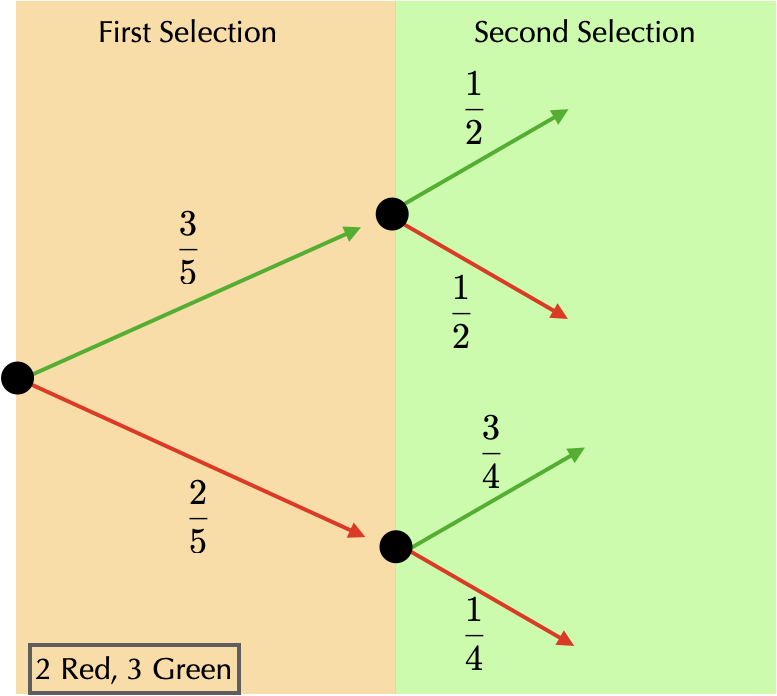
\includegraphics[scale = 0.3]{Figures/treeDiagram.png}
   \caption{Testing \label{fig:tree}}
   \end{figure}

 If event A and B are dependent, then we need to modify equation
 \eqref{eq:orevents} like this:

  \begin{equation}
   P(\text{A or B}) = P(A) + P(B\cap  \text{not A}) - P(A \cap B)\label{eq:oreventsdependent}
 \end{equation}

 A tree diagram (see figure \ref{fig:tree}) will help to understand
 how this works.  On the first selection, the probability of drawing a
 green marble is $P(A) =  {3\over 5}$.  $P(B| \text{not A})$ is the
 probability that a green marble is draw on the second selection
 \underline{assuming that} a green marble was not drawn on the first.
 From the tree diagram we can see that this is equal to:  We can use
 equation \eqref{eq:andprobabilityII} to find $P(B\cap \text{not A})$:

 \begin{align}
   P(B\cap \text{not A}) &= P(B| \text{not A}) \times P(A)\nonumber \\
                         &= {3\over 4} {2\over 5}\nonumber
 \end{align}

 \begin{equation}
   P(A \cap B) = {3\over 5}{1\over 2}\nonumber
\end{equation}

Putting it all together we get:

  \begin{align}
   P(\text{A or B}) &= P(A) + P(B\cap  \text{not A}) - P(A \cap
                      B)\\\nonumber
                      &= {3\over 5} + {3\over 4}{2\over 5} - {3\over 5}{1\over 2}\\\nonumber
                      &= {3\over 5} + {6\over 20} - {3\over 10}\\\nonumber
                      &= {12\over 20} + {6\over 20} - {6\over 20}\\\nonumber
                      &= {12\over 20}\\\nonumber
                      &= {3\over 5}\nonumber
 \end{align}

 Another way to see this result is to enumerate all possible ways to
 draw these marbles from the basket: (There are only ten possible ways
 to do this.)\\

 
\noindent {r, r, g, g, g}\\
 \textcolor{red}{r, g, r, g, g}\\
\textcolor{red} {r, g, g, r, g}\\
 \textcolor{red}{r, g, g, g, r}\\
 \textcolor{red}{g, r, r, g, g}\\
 \textcolor{red}{g, r, g, r, g}\\
 \textcolor{red}{g, r, g, g, r}\\
 {g, g, r, r, g}\\
 {g, g, r, g, r}\\
 {g, g, g, r, r}\\


 And notice that there are 6 ways where one (and only one) of the
 first two selections is green.  Hence, the probability is ${6\over
   10} = {3\over 5}$

\part{Bayesian Statistics}
%\input{chapters/gaussianProcess}
\part{Regression}
\part{Optimization Algorithms}


 Commented out by Michael Ware.  Code below inserts index
 \begin{theindex}
 \documentclass[twoside,11pt,ShortChapTitles]{BYUTextbook}

\usepackage{soul}
\renewcommand{\vec}[1]{\ensuremath{\mathbf{#1}}}
\newcounter{dummy}
\usepackage[style=verbose,backend=bibtex]{biblatex}  % For footnote citations
\addbibresource{refs.bib}
\usepackage[super]{nth}
\newcommand{\labsection}[1]{\refstepcounter{dummy}\addcontentsline{toc}{section}{#1}\section*{#1}}
\usepackage{siunitx}
\sisetup{round-mode = figures,
  round-precision = 3, scientific-notation=true}
\newif\ifsolutions
\solutionsfalse

\begin{document}

\frontmatter

 \thispagestyle{empty}
 \begin{adjustwidth}{}{-1.5in}
 \centering
 {\huge Machine Learning for Physicists}
 %\vskip1.5truein

    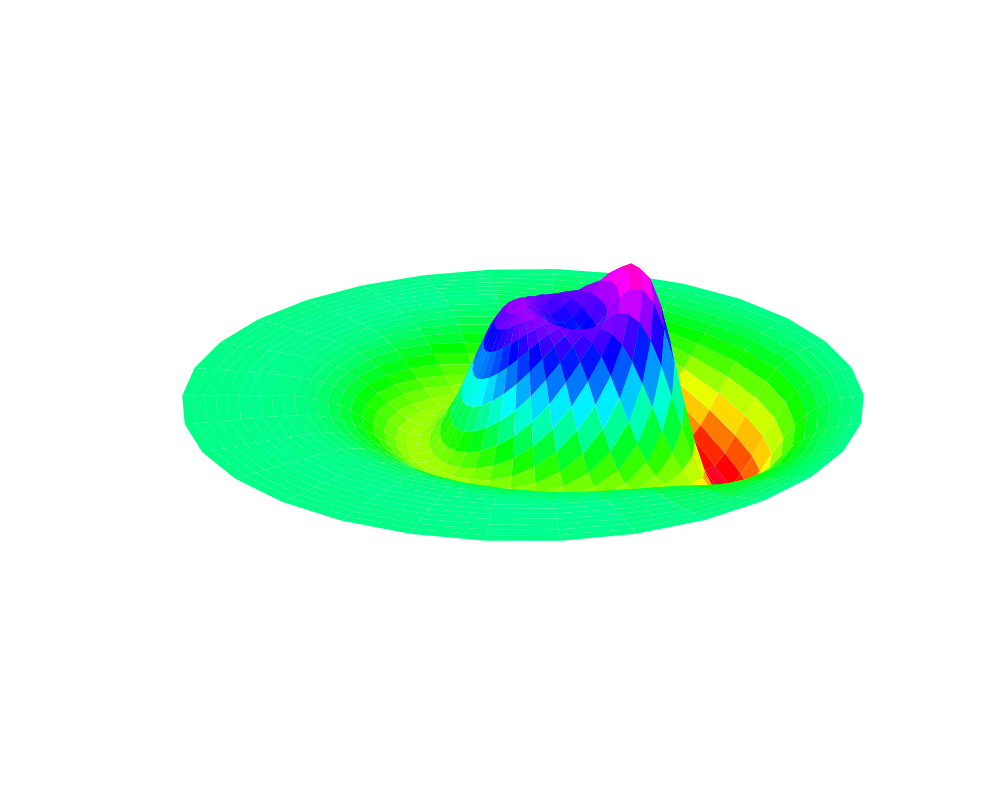
\includegraphics[scale=0.6]{Figures/circMembrane}

%\vskip1truein
Lance J.\ Nelson

\vskip.4truein
Department of Physics
\end{adjustwidth}

\cleardoublepage
\thispagestyle{empty}

 \begin{adjustwidth}{}{-1.5in}
 \centering
 \vspace*{1in}
 \large
 {\huge Machine Learning for Physicists}
 \vskip.4truein

 Lance J.\ Nelson
 \bigskip

 Department of Physics

 \bigskip
 Brigham Young University--Idaho

 \vfill


 {\footnotesize $\copyright$ 2020 Lance J.\ Nelson
               Brigham Young University--Idaho}

 \vskip.5truein
 {\footnotesize \emph{Last Revised: \today}}
 \normalsize

 \end{adjustwidth}

\cleardoublepage
\phantomsection
\chapter*{Preface}

This is a lab notebook intended to give you experience solving
ordinary and partial differential equations numerically.  The
objectives of this course are 
\begin{itemize}
\item to help you learn how to solve a differential equation
  numerically; in situations when a paper-and-pencil solution is
  impossible or impractical.
\item to help you gain greater skills programming a computer and using
  loops, logic, functions, and classes.
\item that your ability to produce a high-quality, professional
  scientific document will increase.
\end{itemize}

Text with a bold P designation (\textbf{P1.1} for example) indicate tasks
that will be done together in class.  Text with a bold H designation
are homework problems and should be completed out of class. (working
in groups is encouraged.) 

Python is the programming language that we will be using You can
obtain a free copy of Python
\href{https://store.enthought.com/downloads/}{here}.  Any computer
code that you create should be uploaded to the Google Drive folder
provided.

There is a companion book to this one entitled, ``Introduction to
Python''.  It is intended to help you learn to use Python to do the
tasks contained herein.  


 \cleardoublepage 
\phantomsection
 \addcontentsline{toc}{chapter}{Table of Contents}
\tableofcontents

\mainmatter
\renewcommand{\chaptermark}[1]{\markboth{Computational Physics 385}{\chaptername \ \thechapter \ \ #1}}
\part{Simple Probability}
\chapter{Introduction to Probability}
 \label{chap:probability} \index{Probability}
 \index{Kernels}

 \labsection{Simple Probability} For most people, the idea of simple
 probability is pretty intuitive.  The probability of rolling a 5 on a
 6-sided die is ${ 1\over 6}$ because of the $6$ possible outcomes,
 only one of them produces a $5$.  The probability of drawing a red
 card in a standard, 52-card deck is ${13\over 52}$ because of the 52
 total cards, $13$ of them are red.  Generalizing this idea yields the
 equation:

\begin{equation}\label{eq:simpleProb}
  P(\text{event~ A}) = {\text{\#~of~ways~A~can~happen}\over \text{Total~\#~of~things~that~could~happen}}
\end{equation}


This equation is the most general version for calculating probability
and is a good one to fall back on when you get stuck.  However,
sometimes it's hard, or impossible, to count the number of possible
outcomes. For example, consider rolling a fair, $6$-sided dice, three
times.  What is the probability that the sum of these three rolls is
less than $10$?  To answer the question using equation
\eqref{eq:simpleProb} you could write down all possible combinations
of three dice rolls (there are 216 of them) and then identify how many
of them summed to a number less than $10$.  While you could probably
write some computer code to do this fairly easily, you probably don't want to do
it by hand. If you're still skeptical, consider increasing the number
of dice rolls to 4 or 5 and reconsider the problem.  It isn't hard to get a
situation where brute-force enumeration and counting is not a great idea.


What follows are some tricks and rules that you can
use to calculate probability when brute-force counting is intractable.


\labsection{Probability of multiple events} 

For example, a single dice roll has $6$ possible outcomes, two dice
rolls has $36$ possible outcomes (illustrated in figure
\ref{twoDieRolls}) and three dice rolls has $216$ possible outcomes.
Clearly you don't want to be enumerating these by hand.  One scenario
where outcome counting becomes challenging is when asking about the
probability of multiple events occuring.  This is because you have to
consider whether the outcome of one event will affect the outcome of
the next.  For example, suppose you roll a $6$-sided die twice and you
want to know the probability that both rolls come up $5$.  Having a
$5$ come up on the first roll doesn't affect the probability that a
$5$ comes up on the second.  These two events are independent of one
another.  The outcome of one event does not affect the outcome of the
other.

In contrast, consider randomly selecting marbles out of a bag which initially
contains $3$ red marbles and $8$ green marbles.  If you reach into the
bag and grab two marbles, what is the probability that they will both
be red?  Notice that selecting a red marble on the first reach into the bag
modifies the number or red marbles available for selection on the
second reach into the bag. Hence the two probabilities are dependent
on each other.  This is an example of dependent events.

\subsection*{Intersection of two events (event A \underline{and} event B)}
\marginfig[-1in]{Figures/twoDieRollsII}{\label{twoDieRolls}All 36
  outcomes from rolling two fair dice.  Out of 36 possible outcomes,
  only one yields a $5$ on both rolls.  Hence the probability of
  rolling two $5$'s is ${1\over 36}$.}

We'll start with the case where two events, $A$ and $B$, both
occur. (Also called the intersection of two events. See figure \ref{fig:VennDiagram})
The math for this sort of situation is:

\begin{equation}
  P(A \cap B) = P(A)  \times P(B)\nonumber
\end{equation}

but let's see some examples so it makes more sense.


\subsubsection*{Independent Events}
Consider rolling a fair $6$-sided dice.  What is the probability that
$5$ comes up on the first two rolls?  Your intuition is probably telling
you that rolling two $5$'s is less likely than rolling just one, so
you expect the probability to be less than ${1\over 6}$.  In figure
\ref{twoDieRolls} you will see all 36 possible outcomes when rolling a
fair dice two times.  Of those 36 possible outcomes how many of
occurrences of two $5$'s being rolled were there?  Just one.  Hence,
the probability is ${1\over 36}$.  You may have noticed that
${1\over 36} = {1\over 6} \times {1\over 6}$.  In other words, the
probability of event A happening \textbf{and} event B happening is
just the product of the two individual probabilities:

\begin{equation}
  P(A\text{ and } B) = P(A) \times P(B)\nonumber
\end{equation}



sometimes $P(A\text{ and } B)$ is written using the symbol for
intersection ($\cap$):
\begin{equation}\label{eq:andprobability}
  P(A \cap B) = P(A) \times P(B)
\end{equation}




\subsubsection{Dependent Events}
When the outcome of one event is affected by the outcome of a previous
event, we say they events are dependent.  For example, consider a bag
containing $3$ red marbles and $8$ green marbles.  If I reach into the
bag and select two marbles, what is the probability that they are both
red.  The probability that my first selection is red is:

\begin{equation}
P(A) = {3\over 11}  \nonumber
\end{equation}

\marginfig[-1in]{Figures/VennDiagram}{\label{fig:VennDiagram}If the
  blue circle represents the probability of A occuring and the red
  circle represents the probability of B occuring, then the overlap of
these two circles is the probability of both events occuring. By
sliding one cirle left or right we can adjust the size of the overlap
(aka $P(A|B)$)}

because $3$ out of the $11$ choices are red.  What about the second
selection?  After the first selection, I am left with $10$ marbles,
$2$ of them being red.  Hence, the probability that I draw a red
marble on my second selection is:

\begin{equation}
 P(B) = {2\over 10}\nonumber
\end{equation}

The probability that my first selection will be a red marble (event A)
\textbf{and} my second selection will also be a red marble (event B)
is then

\begin{align}
  P(A \cap B) &= P(A) \times P(B|A)\nonumber\\
              &= {3\over 11} {2\over 10}\nonumber\\
              &= {6 \over 110}\nonumber\\
              &= 0.055 \nonumber\\
              &= 5.5\%\nonumber
\end{align}

where $P(A|B)$ is called ``conditional probability'' and means the
probability of $B$ happening \textbf{given that} $A$ already happened.

Notice that this is really the same thing we did for independent
events (namely, multiply the two individual probabilities together)
but we just had to be explicit state that when calculating the
probability of event B we had to assume the event A had already happened.

If we want the probility of more than two events happening, we can
continue to multiply conditional probabilities for each event, making
sure to condition it on a positive result for all previous events.

Whether the events are dependent or independent doesn't change the
general equation for multiple events, which is given by equation
\eqref{eq:andprobability}.  However, to account for the possibility
that event B's probability depends on event A, we'll write equation
\eqref{eq:andprobability} as

\begin{equation}\label{eq:andprobabilityII}
  P(A \cap B) = P(A) \times P(B|A)
\end{equation}

where $P(A|B)$ is called ``conditional probability'' and means the
probability of $B$ happening \textbf{given that} $A$ already happened.

We can do a little algebra on equation \eqref{eq:andprobabilityII} to
get:

\begin{equation}
  P(B|A) = {P(A \cap B)\over P(A)}
\end{equation}

Furthermore, if $A$ and $B$ are independent events, then $P(A\cap B) =
P(B \cap A) = P(B) \times P(A|B)$.  Hence, the above equation becomes:

\begin{align}
  P(B|A) &= {P(A \cap B)\over P(A)}\\
         &= \boxed{{P(A|B) P(B) \over P(A)}}
\end{align}


\marginfig[-1in]{Figures/twoDieRollsIII}{\label{fig:twoDieRollsIII}All 36
  outcomes from rolling two fair dice.  <first roll> - <second roll>}

This is known as Bayes' Theorem or Bayes' Rule and is of profound
importance going forward.



\subsection*{Union of two events (event A \underline{or} event B)}
Things change a little if you are asking about the probability that
either event A happens, or event B happens.  Let's handle independent
events first, then we'll do dependent events.

\subsubsection*{Independent Events}
Let's take the dice-rolling example that we've been working with and
ask ourselves what the probability is that either the first roll
is a $5$ \underline{or} the second roll is a $5$.  Figure
\ref{fig:twoDieRollsIII} will help us answer the question and then
we'll try to generalize the result.  The figure shows all possible
results when rolling two fair die.  Highlighted are the cases where
one of the rolls was a 5.  As you can see, there are $11$ ways that
one of the rolls can be a $5$.  Hence, the probability is ${11\over
  36}$.  That's a great way to do a really simple problem, but what if
 I roll the dice 10 times and ask what the probability is that one of
 them is a 5.  Not so easy anymore right.  Let's try to generalize
 this result.  The general equation for \underline{or} events is:

 \begin{equation}
   P(\text{A or B}) = P(A) + P(B) - P(A,B)\label{eq:orevents}
\end{equation}
 
where $P(A)$ is the probability that event A occurs, $P(B)$ is the
probability that event B occurs, and $P(A,B)$ is the probability that
A and B both occur. Let's see what this works out to for this problem:


 \begin{align}
   P(\text{A or B}) &= {1\over 6} + {1\over 6} - {1\over 36}\\
                    &= {6\over 36} + {6\over 36} - {1\over 36}\\
                    &= {11\over 36}\\
 \end{align}

 which agrees with our result from the table.

 \subsubsection*{Dependent Events}

 \begin{figure}
   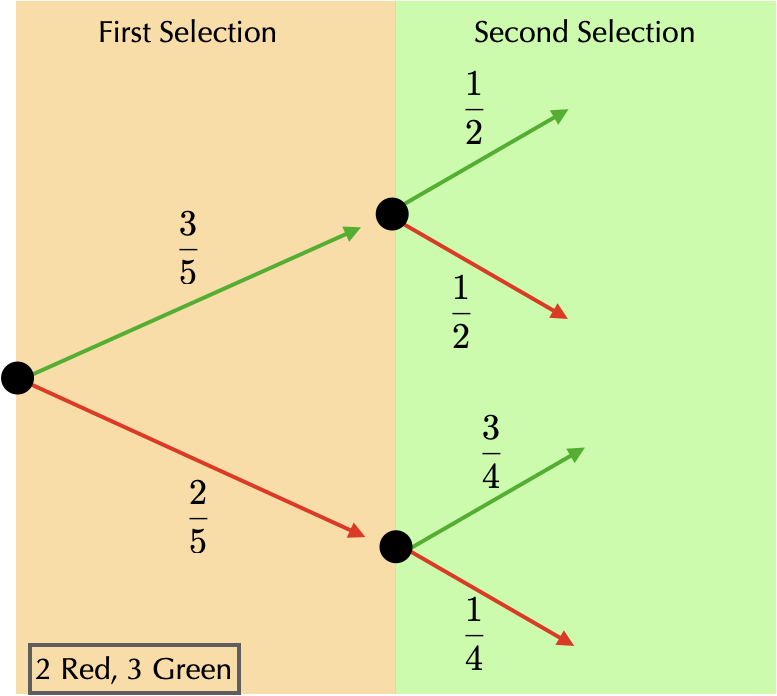
\includegraphics[scale = 0.3]{Figures/treeDiagram.png}
   \caption{Testing \label{fig:tree}}
   \end{figure}

 If event A and B are dependent, then we need to modify equation
 \eqref{eq:orevents} like this:

  \begin{equation}
   P(\text{A or B}) = P(A) + P(B\cap  \text{not A}) - P(A \cap B)\label{eq:oreventsdependent}
 \end{equation}

 A tree diagram (see figure \ref{fig:tree}) will help to understand
 how this works.  On the first selection, the probability of drawing a
 green marble is $P(A) =  {3\over 5}$.  $P(B| \text{not A})$ is the
 probability that a green marble is draw on the second selection
 \underline{assuming that} a green marble was not drawn on the first.
 From the tree diagram we can see that this is equal to:  We can use
 equation \eqref{eq:andprobabilityII} to find $P(B\cap \text{not A})$:

 \begin{align}
   P(B\cap \text{not A}) &= P(B| \text{not A}) \times P(A)\nonumber \\
                         &= {3\over 4} {2\over 5}\nonumber
 \end{align}

 \begin{equation}
   P(A \cap B) = {3\over 5}{1\over 2}\nonumber
\end{equation}

Putting it all together we get:

  \begin{align}
   P(\text{A or B}) &= P(A) + P(B\cap  \text{not A}) - P(A \cap
                      B)\\\nonumber
                      &= {3\over 5} + {3\over 4}{2\over 5} - {3\over 5}{1\over 2}\\\nonumber
                      &= {3\over 5} + {6\over 20} - {3\over 10}\\\nonumber
                      &= {12\over 20} + {6\over 20} - {6\over 20}\\\nonumber
                      &= {12\over 20}\\\nonumber
                      &= {3\over 5}\nonumber
 \end{align}

 Another way to see this result is to enumerate all possible ways to
 draw these marbles from the basket: (There are only ten possible ways
 to do this.)\\

 
\noindent {r, r, g, g, g}\\
 \textcolor{red}{r, g, r, g, g}\\
\textcolor{red} {r, g, g, r, g}\\
 \textcolor{red}{r, g, g, g, r}\\
 \textcolor{red}{g, r, r, g, g}\\
 \textcolor{red}{g, r, g, r, g}\\
 \textcolor{red}{g, r, g, g, r}\\
 {g, g, r, r, g}\\
 {g, g, r, g, r}\\
 {g, g, g, r, r}\\


 And notice that there are 6 ways where one (and only one) of the
 first two selections is green.  Hence, the probability is ${6\over
   10} = {3\over 5}$

\part{Bayesian Statistics}
%\input{chapters/gaussianProcess}
\part{Regression}
\part{Optimization Algorithms}


 Commented out by Michael Ware.  Code below inserts index
 \begin{theindex}
 \documentclass[twoside,11pt,ShortChapTitles]{BYUTextbook}

\usepackage{soul}
\renewcommand{\vec}[1]{\ensuremath{\mathbf{#1}}}
\newcounter{dummy}
\usepackage[style=verbose,backend=bibtex]{biblatex}  % For footnote citations
\addbibresource{refs.bib}
\usepackage[super]{nth}
\newcommand{\labsection}[1]{\refstepcounter{dummy}\addcontentsline{toc}{section}{#1}\section*{#1}}
\usepackage{siunitx}
\sisetup{round-mode = figures,
  round-precision = 3, scientific-notation=true}
\newif\ifsolutions
\solutionsfalse

\begin{document}

\frontmatter

 \thispagestyle{empty}
 \begin{adjustwidth}{}{-1.5in}
 \centering
 {\huge Machine Learning for Physicists}
 %\vskip1.5truein

    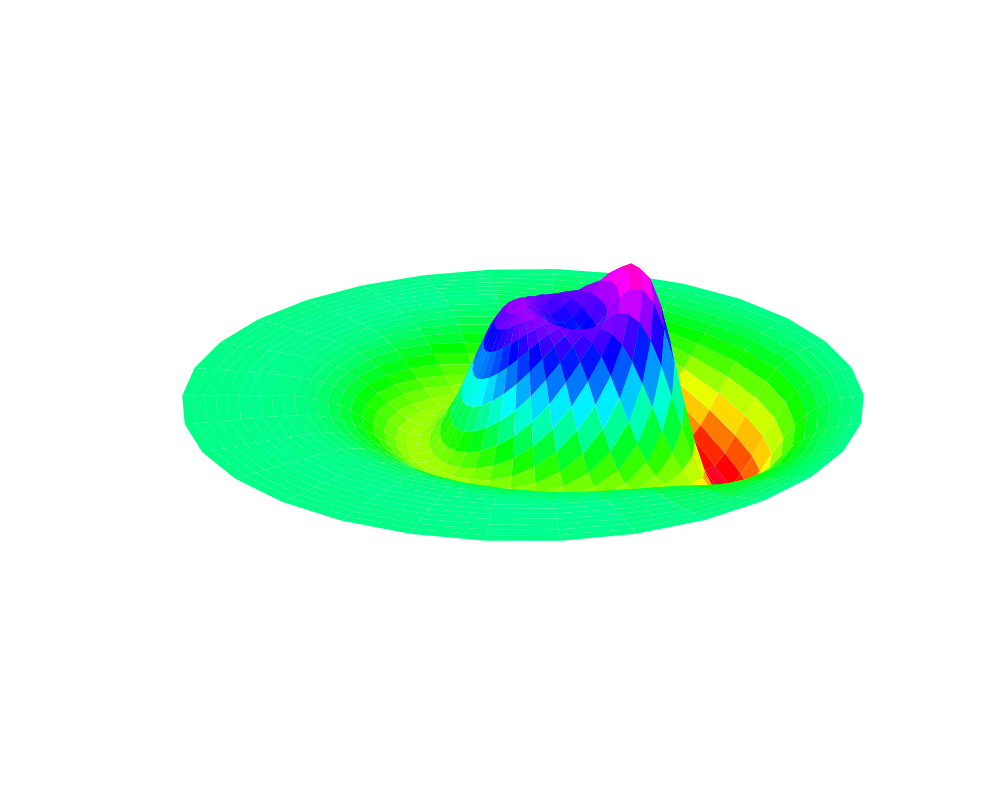
\includegraphics[scale=0.6]{Figures/circMembrane}

%\vskip1truein
Lance J.\ Nelson

\vskip.4truein
Department of Physics
\end{adjustwidth}

\cleardoublepage
\thispagestyle{empty}

 \begin{adjustwidth}{}{-1.5in}
 \centering
 \vspace*{1in}
 \large
 {\huge Machine Learning for Physicists}
 \vskip.4truein

 Lance J.\ Nelson
 \bigskip

 Department of Physics

 \bigskip
 Brigham Young University--Idaho

 \vfill


 {\footnotesize $\copyright$ 2020 Lance J.\ Nelson
               Brigham Young University--Idaho}

 \vskip.5truein
 {\footnotesize \emph{Last Revised: \today}}
 \normalsize

 \end{adjustwidth}

\cleardoublepage
\phantomsection
\chapter*{Preface}

This is a lab notebook intended to give you experience solving
ordinary and partial differential equations numerically.  The
objectives of this course are 
\begin{itemize}
\item to help you learn how to solve a differential equation
  numerically; in situations when a paper-and-pencil solution is
  impossible or impractical.
\item to help you gain greater skills programming a computer and using
  loops, logic, functions, and classes.
\item that your ability to produce a high-quality, professional
  scientific document will increase.
\end{itemize}

Text with a bold P designation (\textbf{P1.1} for example) indicate tasks
that will be done together in class.  Text with a bold H designation
are homework problems and should be completed out of class. (working
in groups is encouraged.) 

Python is the programming language that we will be using You can
obtain a free copy of Python
\href{https://store.enthought.com/downloads/}{here}.  Any computer
code that you create should be uploaded to the Google Drive folder
provided.

There is a companion book to this one entitled, ``Introduction to
Python''.  It is intended to help you learn to use Python to do the
tasks contained herein.  


 \cleardoublepage 
\phantomsection
 \addcontentsline{toc}{chapter}{Table of Contents}
\tableofcontents

\mainmatter
\renewcommand{\chaptermark}[1]{\markboth{Computational Physics 385}{\chaptername \ \thechapter \ \ #1}}
\part{Simple Probability}
\chapter{Introduction to Probability}
 \label{chap:probability} \index{Probability}
 \index{Kernels}

 \labsection{Simple Probability} For most people, the idea of simple
 probability is pretty intuitive.  The probability of rolling a 5 on a
 6-sided die is ${ 1\over 6}$ because of the $6$ possible outcomes,
 only one of them produces a $5$.  The probability of drawing a red
 card in a standard, 52-card deck is ${13\over 52}$ because of the 52
 total cards, $13$ of them are red.  Generalizing this idea yields the
 equation:

\begin{equation}\label{eq:simpleProb}
  P(\text{event~ A}) = {\text{\#~of~ways~A~can~happen}\over \text{Total~\#~of~things~that~could~happen}}
\end{equation}


This equation is the most general version for calculating probability
and is a good one to fall back on when you get stuck.  However,
sometimes it's hard, or impossible, to count the number of possible
outcomes. For example, consider rolling a fair, $6$-sided dice, three
times.  What is the probability that the sum of these three rolls is
less than $10$?  To answer the question using equation
\eqref{eq:simpleProb} you could write down all possible combinations
of three dice rolls (there are 216 of them) and then identify how many
of them summed to a number less than $10$.  While you could probably
write some computer code to do this fairly easily, you probably don't want to do
it by hand. If you're still skeptical, consider increasing the number
of dice rolls to 4 or 5 and reconsider the problem.  It isn't hard to get a
situation where brute-force enumeration and counting is not a great idea.


What follows are some tricks and rules that you can
use to calculate probability when brute-force counting is intractable.


\labsection{Probability of multiple events} 

For example, a single dice roll has $6$ possible outcomes, two dice
rolls has $36$ possible outcomes (illustrated in figure
\ref{twoDieRolls}) and three dice rolls has $216$ possible outcomes.
Clearly you don't want to be enumerating these by hand.  One scenario
where outcome counting becomes challenging is when asking about the
probability of multiple events occuring.  This is because you have to
consider whether the outcome of one event will affect the outcome of
the next.  For example, suppose you roll a $6$-sided die twice and you
want to know the probability that both rolls come up $5$.  Having a
$5$ come up on the first roll doesn't affect the probability that a
$5$ comes up on the second.  These two events are independent of one
another.  The outcome of one event does not affect the outcome of the
other.

In contrast, consider randomly selecting marbles out of a bag which initially
contains $3$ red marbles and $8$ green marbles.  If you reach into the
bag and grab two marbles, what is the probability that they will both
be red?  Notice that selecting a red marble on the first reach into the bag
modifies the number or red marbles available for selection on the
second reach into the bag. Hence the two probabilities are dependent
on each other.  This is an example of dependent events.

\subsection*{Intersection of two events (event A \underline{and} event B)}
\marginfig[-1in]{Figures/twoDieRollsII}{\label{twoDieRolls}All 36
  outcomes from rolling two fair dice.  Out of 36 possible outcomes,
  only one yields a $5$ on both rolls.  Hence the probability of
  rolling two $5$'s is ${1\over 36}$.}

We'll start with the case where two events, $A$ and $B$, both
occur. (Also called the intersection of two events. See figure \ref{fig:VennDiagram})
The math for this sort of situation is:

\begin{equation}
  P(A \cap B) = P(A)  \times P(B)\nonumber
\end{equation}

but let's see some examples so it makes more sense.


\subsubsection*{Independent Events}
Consider rolling a fair $6$-sided dice.  What is the probability that
$5$ comes up on the first two rolls?  Your intuition is probably telling
you that rolling two $5$'s is less likely than rolling just one, so
you expect the probability to be less than ${1\over 6}$.  In figure
\ref{twoDieRolls} you will see all 36 possible outcomes when rolling a
fair dice two times.  Of those 36 possible outcomes how many of
occurrences of two $5$'s being rolled were there?  Just one.  Hence,
the probability is ${1\over 36}$.  You may have noticed that
${1\over 36} = {1\over 6} \times {1\over 6}$.  In other words, the
probability of event A happening \textbf{and} event B happening is
just the product of the two individual probabilities:

\begin{equation}
  P(A\text{ and } B) = P(A) \times P(B)\nonumber
\end{equation}



sometimes $P(A\text{ and } B)$ is written using the symbol for
intersection ($\cap$):
\begin{equation}\label{eq:andprobability}
  P(A \cap B) = P(A) \times P(B)
\end{equation}




\subsubsection{Dependent Events}
When the outcome of one event is affected by the outcome of a previous
event, we say they events are dependent.  For example, consider a bag
containing $3$ red marbles and $8$ green marbles.  If I reach into the
bag and select two marbles, what is the probability that they are both
red.  The probability that my first selection is red is:

\begin{equation}
P(A) = {3\over 11}  \nonumber
\end{equation}

\marginfig[-1in]{Figures/VennDiagram}{\label{fig:VennDiagram}If the
  blue circle represents the probability of A occuring and the red
  circle represents the probability of B occuring, then the overlap of
these two circles is the probability of both events occuring. By
sliding one cirle left or right we can adjust the size of the overlap
(aka $P(A|B)$)}

because $3$ out of the $11$ choices are red.  What about the second
selection?  After the first selection, I am left with $10$ marbles,
$2$ of them being red.  Hence, the probability that I draw a red
marble on my second selection is:

\begin{equation}
 P(B) = {2\over 10}\nonumber
\end{equation}

The probability that my first selection will be a red marble (event A)
\textbf{and} my second selection will also be a red marble (event B)
is then

\begin{align}
  P(A \cap B) &= P(A) \times P(B|A)\nonumber\\
              &= {3\over 11} {2\over 10}\nonumber\\
              &= {6 \over 110}\nonumber\\
              &= 0.055 \nonumber\\
              &= 5.5\%\nonumber
\end{align}

where $P(A|B)$ is called ``conditional probability'' and means the
probability of $B$ happening \textbf{given that} $A$ already happened.

Notice that this is really the same thing we did for independent
events (namely, multiply the two individual probabilities together)
but we just had to be explicit state that when calculating the
probability of event B we had to assume the event A had already happened.

If we want the probility of more than two events happening, we can
continue to multiply conditional probabilities for each event, making
sure to condition it on a positive result for all previous events.

Whether the events are dependent or independent doesn't change the
general equation for multiple events, which is given by equation
\eqref{eq:andprobability}.  However, to account for the possibility
that event B's probability depends on event A, we'll write equation
\eqref{eq:andprobability} as

\begin{equation}\label{eq:andprobabilityII}
  P(A \cap B) = P(A) \times P(B|A)
\end{equation}

where $P(A|B)$ is called ``conditional probability'' and means the
probability of $B$ happening \textbf{given that} $A$ already happened.

We can do a little algebra on equation \eqref{eq:andprobabilityII} to
get:

\begin{equation}
  P(B|A) = {P(A \cap B)\over P(A)}
\end{equation}

Furthermore, if $A$ and $B$ are independent events, then $P(A\cap B) =
P(B \cap A) = P(B) \times P(A|B)$.  Hence, the above equation becomes:

\begin{align}
  P(B|A) &= {P(A \cap B)\over P(A)}\\
         &= \boxed{{P(A|B) P(B) \over P(A)}}
\end{align}


\marginfig[-1in]{Figures/twoDieRollsIII}{\label{fig:twoDieRollsIII}All 36
  outcomes from rolling two fair dice.  <first roll> - <second roll>}

This is known as Bayes' Theorem or Bayes' Rule and is of profound
importance going forward.



\subsection*{Union of two events (event A \underline{or} event B)}
Things change a little if you are asking about the probability that
either event A happens, or event B happens.  Let's handle independent
events first, then we'll do dependent events.

\subsubsection*{Independent Events}
Let's take the dice-rolling example that we've been working with and
ask ourselves what the probability is that either the first roll
is a $5$ \underline{or} the second roll is a $5$.  Figure
\ref{fig:twoDieRollsIII} will help us answer the question and then
we'll try to generalize the result.  The figure shows all possible
results when rolling two fair die.  Highlighted are the cases where
one of the rolls was a 5.  As you can see, there are $11$ ways that
one of the rolls can be a $5$.  Hence, the probability is ${11\over
  36}$.  That's a great way to do a really simple problem, but what if
 I roll the dice 10 times and ask what the probability is that one of
 them is a 5.  Not so easy anymore right.  Let's try to generalize
 this result.  The general equation for \underline{or} events is:

 \begin{equation}
   P(\text{A or B}) = P(A) + P(B) - P(A,B)\label{eq:orevents}
\end{equation}
 
where $P(A)$ is the probability that event A occurs, $P(B)$ is the
probability that event B occurs, and $P(A,B)$ is the probability that
A and B both occur. Let's see what this works out to for this problem:


 \begin{align}
   P(\text{A or B}) &= {1\over 6} + {1\over 6} - {1\over 36}\\
                    &= {6\over 36} + {6\over 36} - {1\over 36}\\
                    &= {11\over 36}\\
 \end{align}

 which agrees with our result from the table.

 \subsubsection*{Dependent Events}

 \begin{figure}
   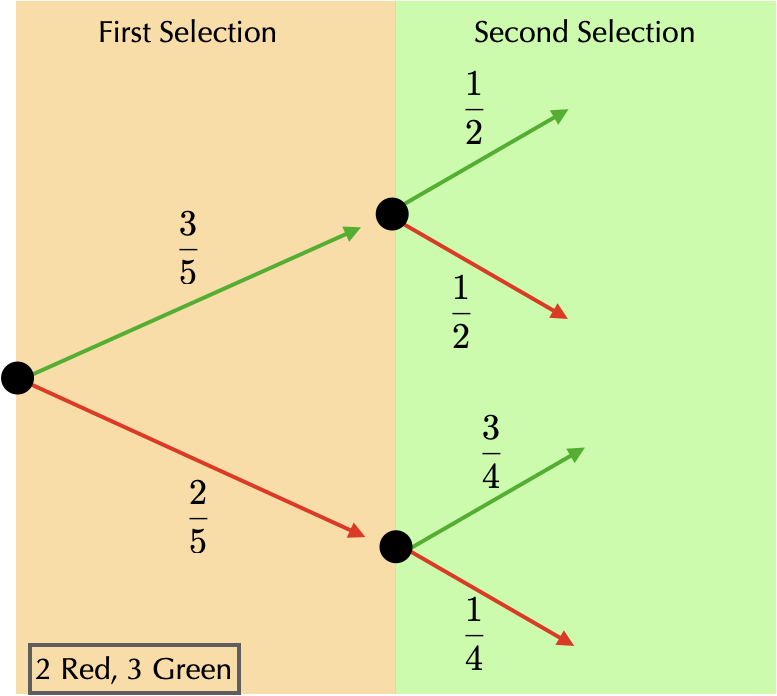
\includegraphics[scale = 0.3]{Figures/treeDiagram.png}
   \caption{Testing \label{fig:tree}}
   \end{figure}

 If event A and B are dependent, then we need to modify equation
 \eqref{eq:orevents} like this:

  \begin{equation}
   P(\text{A or B}) = P(A) + P(B\cap  \text{not A}) - P(A \cap B)\label{eq:oreventsdependent}
 \end{equation}

 A tree diagram (see figure \ref{fig:tree}) will help to understand
 how this works.  On the first selection, the probability of drawing a
 green marble is $P(A) =  {3\over 5}$.  $P(B| \text{not A})$ is the
 probability that a green marble is draw on the second selection
 \underline{assuming that} a green marble was not drawn on the first.
 From the tree diagram we can see that this is equal to:  We can use
 equation \eqref{eq:andprobabilityII} to find $P(B\cap \text{not A})$:

 \begin{align}
   P(B\cap \text{not A}) &= P(B| \text{not A}) \times P(A)\nonumber \\
                         &= {3\over 4} {2\over 5}\nonumber
 \end{align}

 \begin{equation}
   P(A \cap B) = {3\over 5}{1\over 2}\nonumber
\end{equation}

Putting it all together we get:

  \begin{align}
   P(\text{A or B}) &= P(A) + P(B\cap  \text{not A}) - P(A \cap
                      B)\\\nonumber
                      &= {3\over 5} + {3\over 4}{2\over 5} - {3\over 5}{1\over 2}\\\nonumber
                      &= {3\over 5} + {6\over 20} - {3\over 10}\\\nonumber
                      &= {12\over 20} + {6\over 20} - {6\over 20}\\\nonumber
                      &= {12\over 20}\\\nonumber
                      &= {3\over 5}\nonumber
 \end{align}

 Another way to see this result is to enumerate all possible ways to
 draw these marbles from the basket: (There are only ten possible ways
 to do this.)\\

 
\noindent {r, r, g, g, g}\\
 \textcolor{red}{r, g, r, g, g}\\
\textcolor{red} {r, g, g, r, g}\\
 \textcolor{red}{r, g, g, g, r}\\
 \textcolor{red}{g, r, r, g, g}\\
 \textcolor{red}{g, r, g, r, g}\\
 \textcolor{red}{g, r, g, g, r}\\
 {g, g, r, r, g}\\
 {g, g, r, g, r}\\
 {g, g, g, r, r}\\


 And notice that there are 6 ways where one (and only one) of the
 first two selections is green.  Hence, the probability is ${6\over
   10} = {3\over 5}$

\part{Bayesian Statistics}
%\input{chapters/gaussianProcess}
\part{Regression}
\part{Optimization Algorithms}


 Commented out by Michael Ware.  Code below inserts index
 \begin{theindex}
 \documentclass[twoside,11pt,ShortChapTitles]{BYUTextbook}

\usepackage{soul}
\renewcommand{\vec}[1]{\ensuremath{\mathbf{#1}}}
\newcounter{dummy}
\usepackage[style=verbose,backend=bibtex]{biblatex}  % For footnote citations
\addbibresource{refs.bib}
\usepackage[super]{nth}
\newcommand{\labsection}[1]{\refstepcounter{dummy}\addcontentsline{toc}{section}{#1}\section*{#1}}
\usepackage{siunitx}
\sisetup{round-mode = figures,
  round-precision = 3, scientific-notation=true}
\newif\ifsolutions
\solutionsfalse

\begin{document}

\frontmatter

 \thispagestyle{empty}
 \begin{adjustwidth}{}{-1.5in}
 \centering
 {\huge Machine Learning for Physicists}
 %\vskip1.5truein

    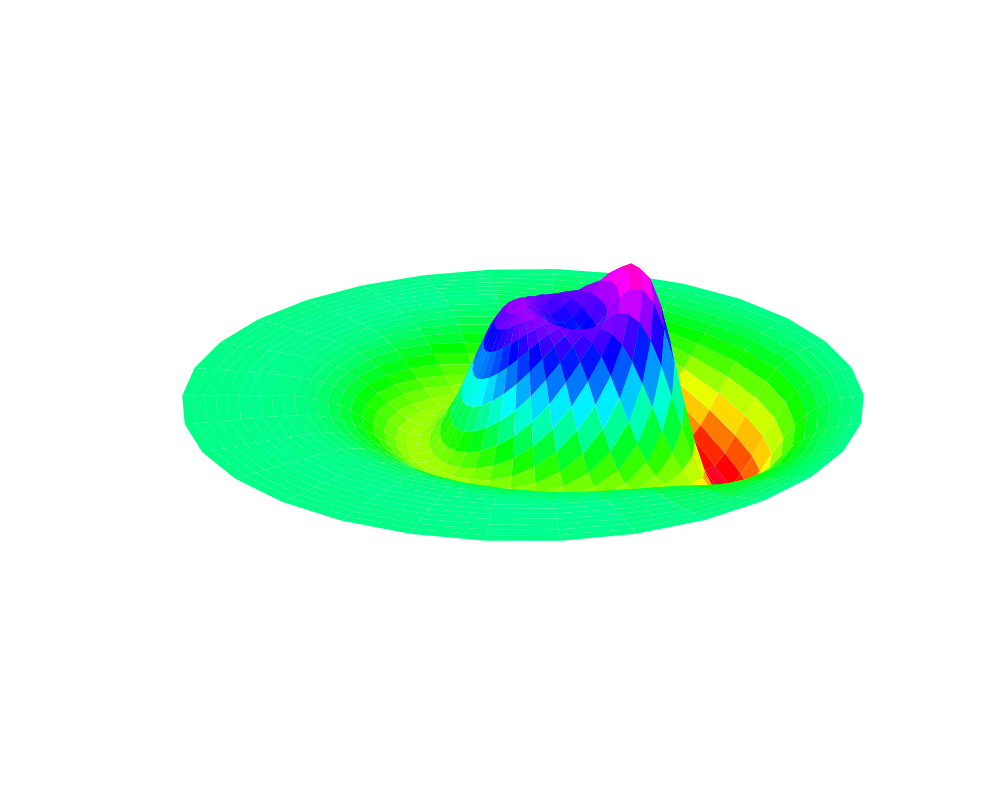
\includegraphics[scale=0.6]{Figures/circMembrane}

%\vskip1truein
Lance J.\ Nelson

\vskip.4truein
Department of Physics
\end{adjustwidth}

\cleardoublepage
\thispagestyle{empty}

 \begin{adjustwidth}{}{-1.5in}
 \centering
 \vspace*{1in}
 \large
 {\huge Machine Learning for Physicists}
 \vskip.4truein

 Lance J.\ Nelson
 \bigskip

 Department of Physics

 \bigskip
 Brigham Young University--Idaho

 \vfill


 {\footnotesize $\copyright$ 2020 Lance J.\ Nelson
               Brigham Young University--Idaho}

 \vskip.5truein
 {\footnotesize \emph{Last Revised: \today}}
 \normalsize

 \end{adjustwidth}

\cleardoublepage
\phantomsection
\input{chapters/preface}


 \cleardoublepage 
\phantomsection
 \addcontentsline{toc}{chapter}{Table of Contents}
\tableofcontents

\mainmatter
\renewcommand{\chaptermark}[1]{\markboth{Computational Physics 385}{\chaptername \ \thechapter \ \ #1}}
\part{Simple Probability}
\input{chapters/probability}
\part{Bayesian Statistics}
%\input{chapters/gaussianProcess}
\part{Regression}
\part{Optimization Algorithms}


 Commented out by Michael Ware.  Code below inserts index
 \begin{theindex}
 \input{MachineLearning.idx}
 \end{theindex}

%\bibliographystyle{ieeetr}
%\bibliography{refs}

 \cleardoublepage \phantomsection
 \addcontentsline{toc}{chapter}{Index}
 \printindex
\printbibliography
\end{document}


 \end{theindex}

%\bibliographystyle{ieeetr}
%\bibliography{refs}

 \cleardoublepage \phantomsection
 \addcontentsline{toc}{chapter}{Index}
 \printindex
\printbibliography
\end{document}


 \end{theindex}

%\bibliographystyle{ieeetr}
%\bibliography{refs}

 \cleardoublepage \phantomsection
 \addcontentsline{toc}{chapter}{Index}
 \printindex
\printbibliography
\end{document}


 \end{theindex}

%\bibliographystyle{ieeetr}
%\bibliography{refs}

 \cleardoublepage \phantomsection
 \addcontentsline{toc}{chapter}{Index}
 \printindex
\printbibliography
\end{document}

